\section{Design}

Argus is designed as a full-screen application to utilise maximum screen space. The application is designed to be keyboard-driven, so shortcuts are displayed wherever possible. Additionally, the current instruction of the workflow is indicated on the top of the image in red to stand out to image taggers. \cref{fig:dataset:argus:overview} shows the main \gls{ui}. Further segment-level features are captured in dialogs or user interaction directly on the image, as shown in \cref{fig:dataset:argus:bib_and_face,fig:dataset:argus:prom_and_col}.

\begin{figure}[h]
  \centering
  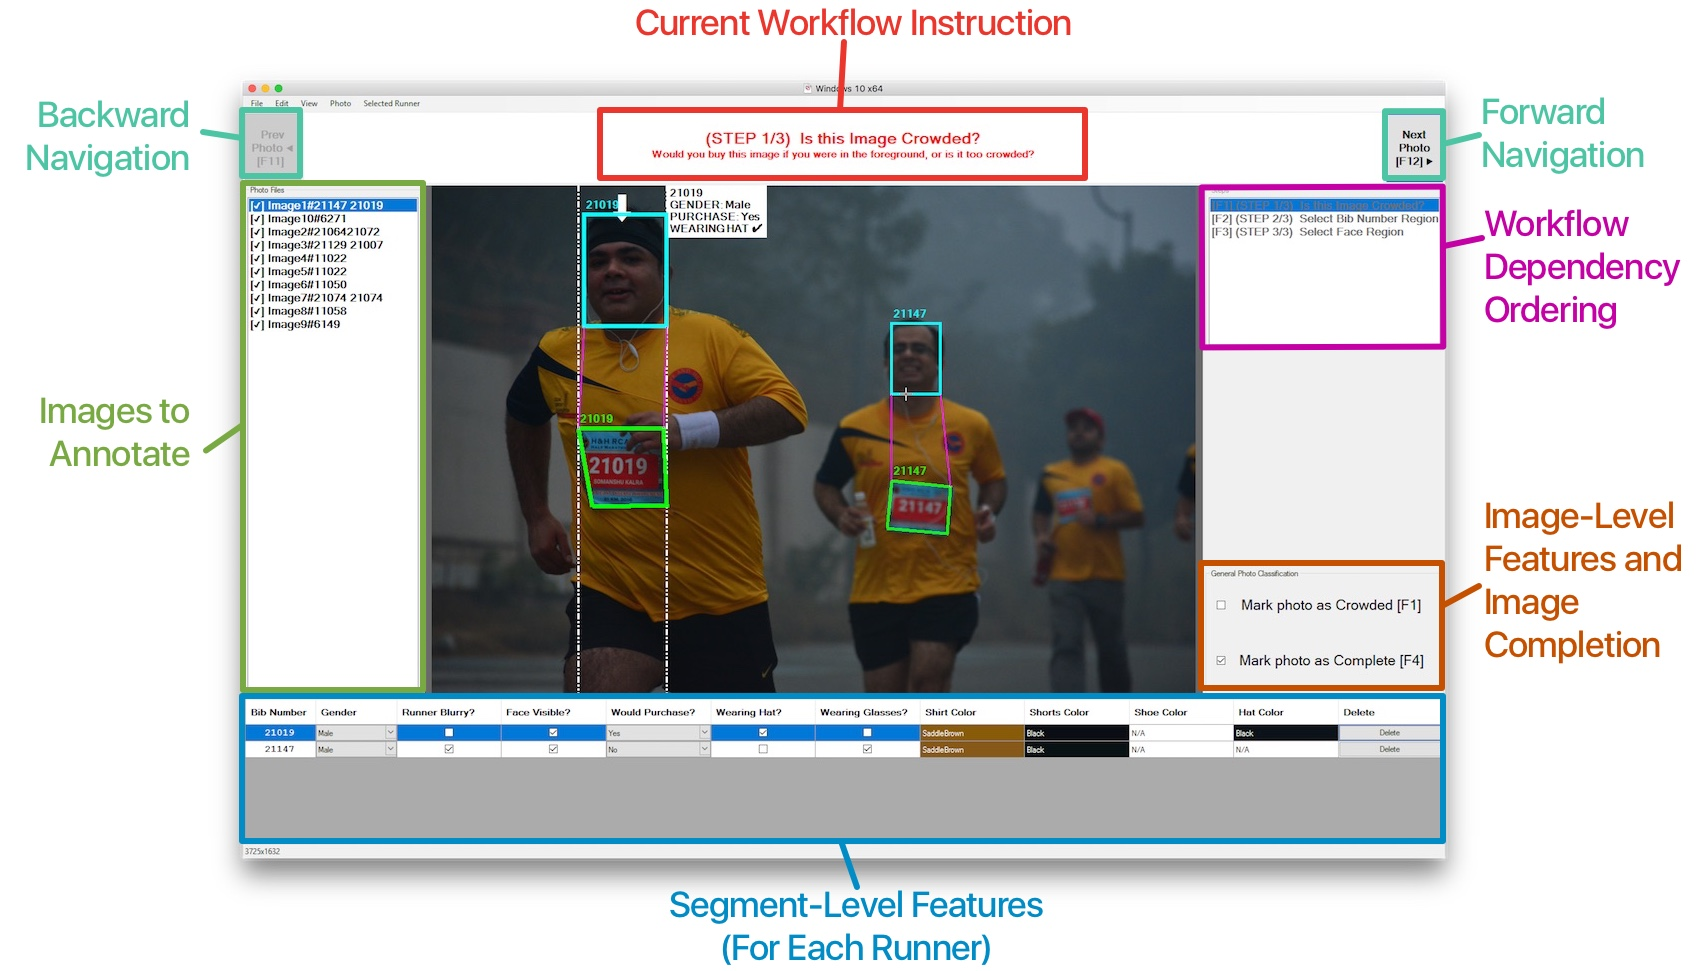
\includegraphics[width=\textwidth]{images/dataset/argus/argus_ui}
  \caption[An overview of the Argus user interface]{An overview of the Argus user interface.}
  \label{fig:dataset:argus:overview}
\end{figure}

\begin{figure}
  \centering
  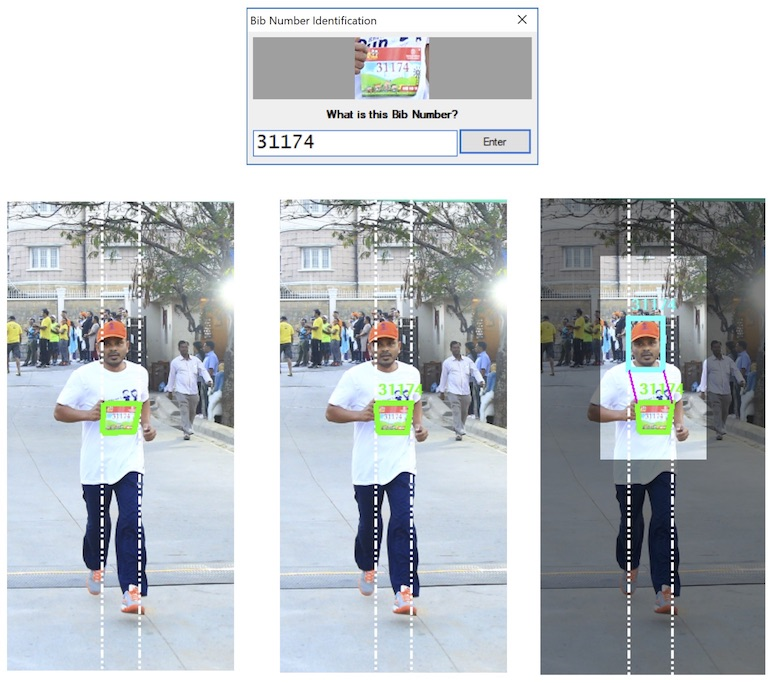
\includegraphics[width=\textwidth]{images/dataset/argus/argus_entry}
  \caption[Bib and Face feature annotation with Argus]{$Bib$ and $Face$ segment-level feature annotation. Users click four times around the bib to mark up the $BibSheet$ region (left). A dialog asks the user to enter the $\gls{rbn}$ label (top). The \gls{rbn} is annotated on the image (middle) and users can progress to drag-and-drop around the $Face$ region within the restrictions set (see \cref{sec:dataset:architecture:metamodel}). Note the dependency ordering is present.}
  \label{fig:dataset:argus:bib_and_face}
\end{figure}

\begin{figure}
  \hspace{\fill}
  \begin{subfigure}[b]{0.45\textwidth}
    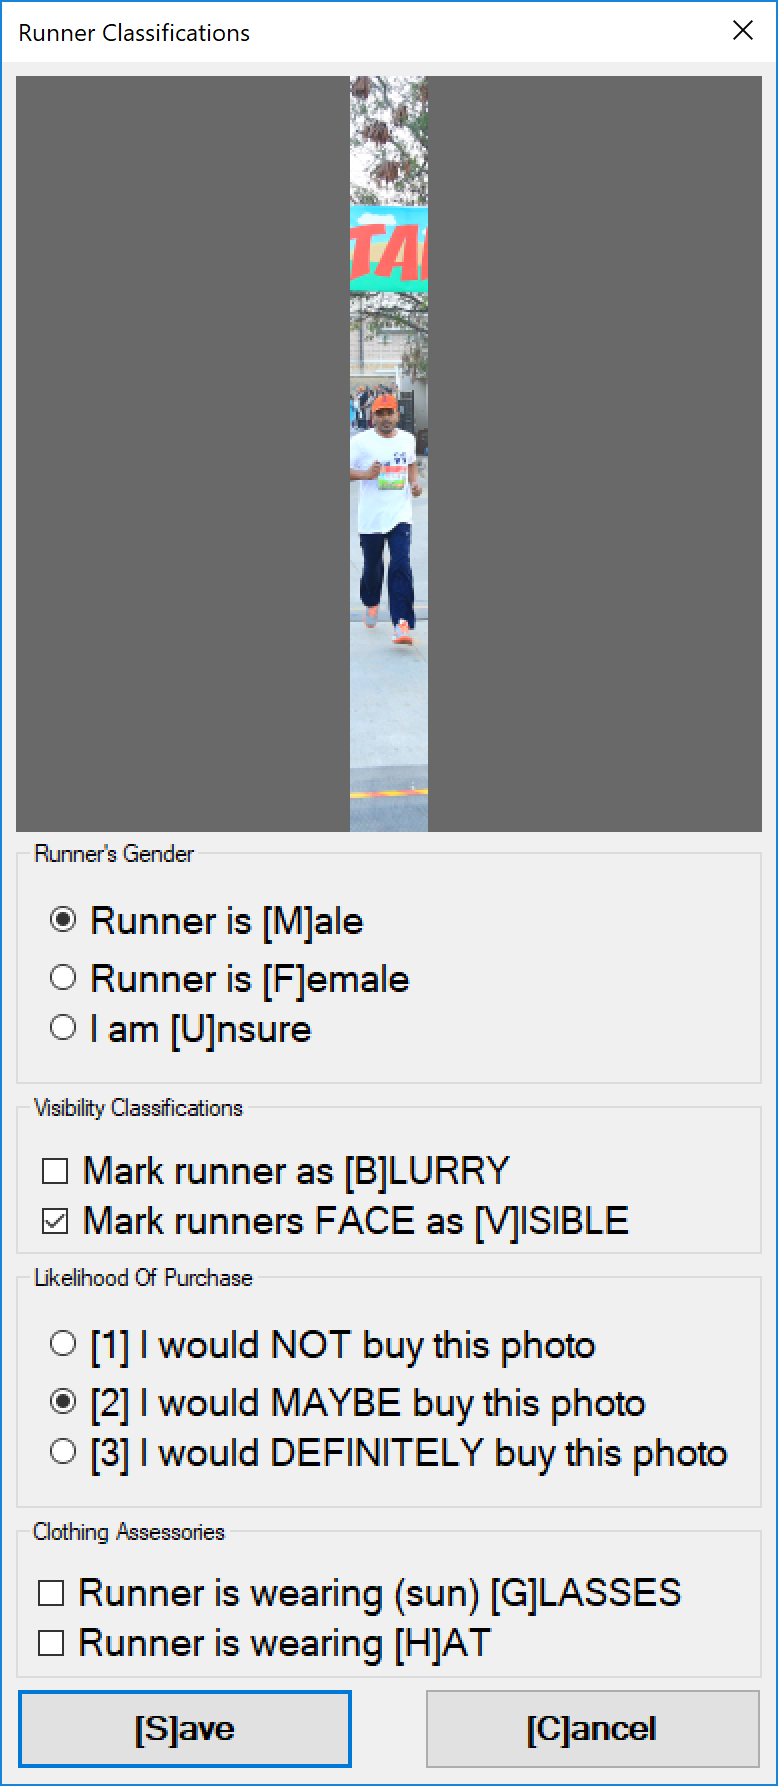
\includegraphics[width=\textwidth]{images/dataset/argus/argus_prom_entry}
  \end{subfigure}
  \hspace{\fill}
  \begin{subfigure}[b]{0.45\textwidth}
    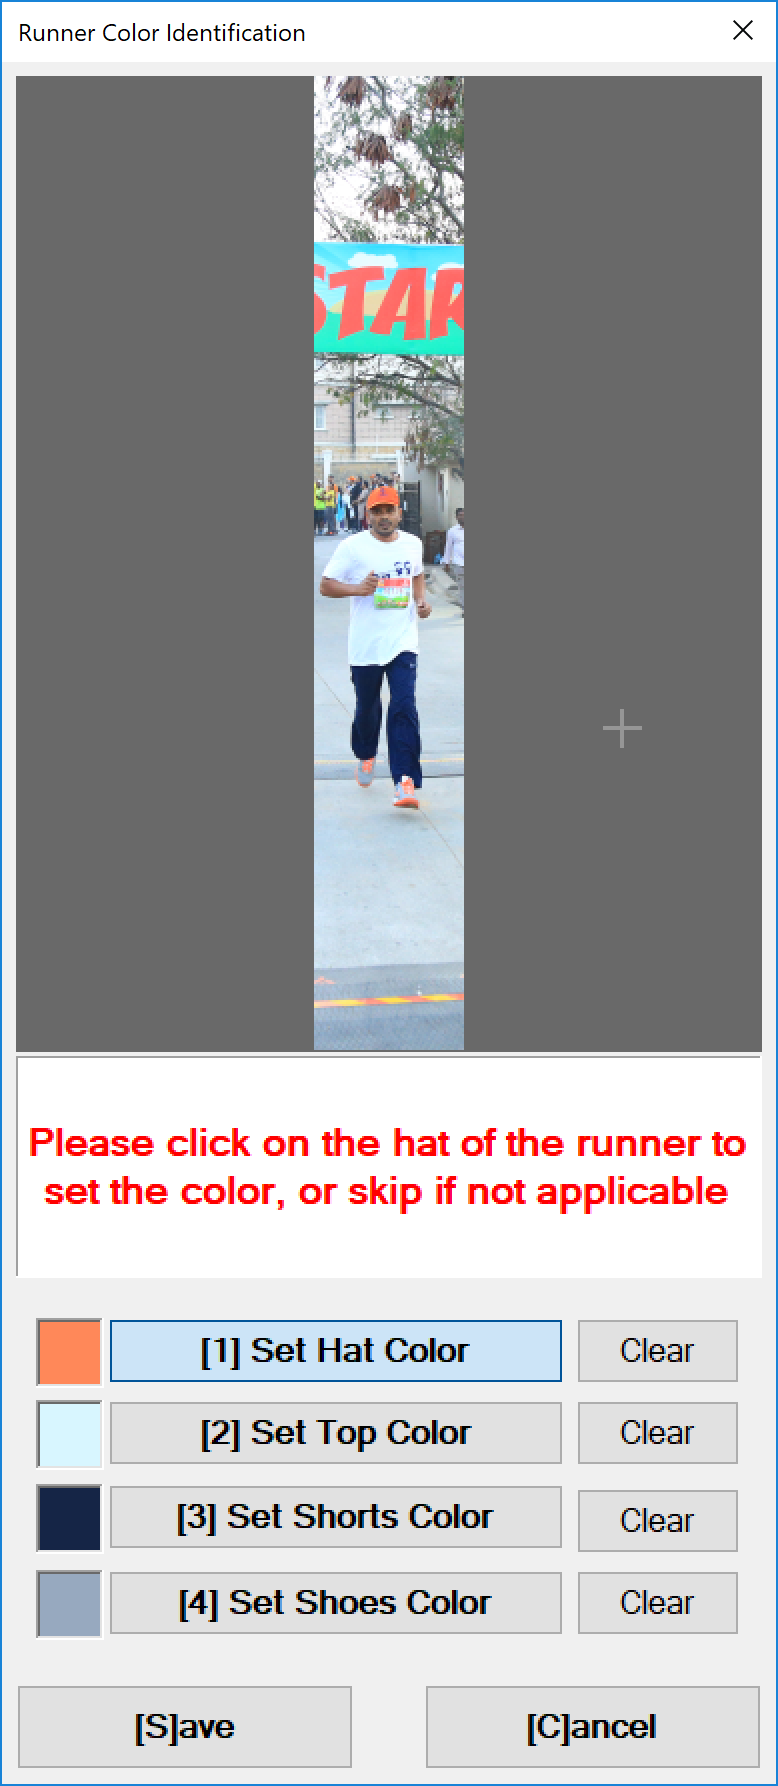
\includegraphics[width=\textwidth]{images/dataset/argus/argus_color_entry}
  \end{subfigure}
  \hspace{\fill}
  \caption[Prominence and Colour feature annotation with Argus]{Annotation for the $Prominence$ and $Colour$ segment-level features.}
  \label{fig:dataset:argus:prom_and_col}
\end{figure}

We deployed Argus to data taggers remotely using the ClickOnce Deployment\footnoteurl{https://msdn.microsoft.com/en-us/library/t71a733d.aspx}{11 August 2017} strategy.